\documentclass{article}                     % onecolumn (standard format)

\usepackage{graphicx}
\usepackage{float}
\usepackage{amsmath}
\usepackage{cite}
\usepackage{subcaption}
\usepackage{rotating}
\usepackage[left=2.2cm, right=2.2cm]{geometry}
\usepackage{algpseudocode}
\usepackage{algorithm}
%\floatstyle{ruled}
\usepackage{hyperref}
\usepackage{algpseudocode}

\usepackage{tikz}
\usetikzlibrary{positioning,calc,shapes,shapes.geometric}
\usepackage{pgf}

\newfloat{algorithm}{tbp}{loa}
\providecommand{\algorithmname}{Algorithm}
\floatname{algorithm}{\protect\algorithmname}


%\renewcommand{\thesection}{\Roman{section}}
\usepackage{titlesec}
\titleformat{\section}
{\normalfont\Large\bfseries}{Exercise~\thesection}{1em}{}

\newfloat{algorithm}{tbp}{loa}
\providecommand{\algorithmname}{Algorithm}
\floatname{algorithm}{\protect\algorithmname}
%
% \usepackage{mathptmx}      % use Times fonts if available on your TeX system
%
% insert here the call for the packages your document requires
%\usepackage{latexsym}
% etc.
%
% please place your own definitions here and don't use \def but
% \newcommand{}{}
%

%
\begin{document}
	
	\title{Introduction to AI - assignment 3}
	
	
	\author{Oded~Yechiel}
	
	\date{27/11/18}
	
	\maketitle
	
	\section{Agents and environment simulators}
	\subsection{An agent that plays Whist}
	Whist is a zero-sum adversarial game. The environment is static and discrete, non observed and non deterministic. There are many possible goal states, and the agent should maximize its own performance while minimizing the performance of the adversarial agent. Therefore, a \textbf{utility-based agent} will best assess the situation and provide the ultimate action.
	\subsection{An agent that can solve Sokoban problems}
	Sokoban is a single player puzzle-like game with a single goal state. The environment is static, discrete, fully observable and deterministic. Therefore, a \textbf{goal-based agent} will be most suitable than all other agents.
	\subsection{An autonomous humanoid robot that can win the DARPA robotics challenge}
	The DRC's task require the robot to perform a series of tasks. Although points are distributed per task, such as, go through the gate, enter the car, drive the car and exit the car, these are merely subgoals and are sequential. Therefore, it would be most logical of using a \textbf{goal-based agent}. The environment is static, continuous, discrete and partially observable.
	\subsection{An internet shopping agent specializing in trip planning}
	An internet shopping agent has many goals, with various optimizing criteria, such as time, cost and comfort. The environment \textbf{may be} considered as a deterministic, fully observable (after query the agent has all of the information) single operating agent (assuming tickets are not running out). Since there is no one perfect goal, the agent should be \textbf{utility-based agent.}
	\subsection{An agent that can play Go}
	Go is a fully observable, non-deterministic, static adversarial game. Although there is only one winner and a definite goal state, it is unlikely for any agent to calculate so deeply into the game and find the optimal action. Therefore, for a given action it is required to assess the situation and decide what action is sub-optimal for the problem. Therefore, a \textbf{utility-based agent} is advised.
	
	\section{Search}
	In the hurricane environment, shown in Fig.~\ref{fig:environment}, there are many different ways in which it is possible to calculate the heuristics of an action. The half-star heuristic, $ h' $ calculates the performance by locating the vertex with most un-savable people and multiplying them by a large number. In this exercise  we shall multiply each person by 100 for ease of calculation and distinction, although multiplying by the "Deadline value" is sufficient.
	
	\begin{figure}
		\centering
		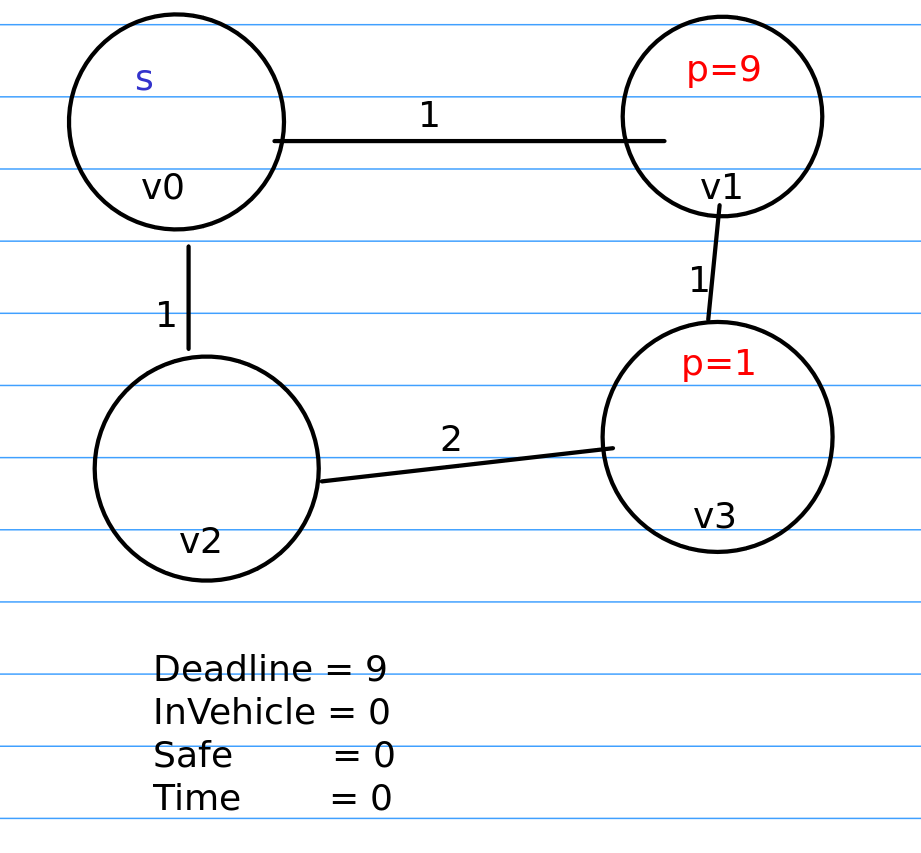
\includegraphics[width=0.5\linewidth]{environment}
		\caption{The hurricane environment.}
		\label{fig:environment}
	\end{figure}
	
	
	We can examine an example of calculating the heuristics for the starting location. The agent is at $ V_0 $ and it is possible to go to $ V_1 $ or $ V_2 $. The heuristic for going to $ V_1 $ will be 100, since we have picked up all the 9 people in $ V_1 $ and the only town with people is $ V_3 $ with 1 person. Going to $ V_2 $ will result in a heuristic of 900, since in $ V_1 $ there are 9 people which are un-savable.
	
	
	\subsection{Greedy agent}
	From the example above, the greedy agent will obviously prefer going to $ V_1 $, even-though it is obvious that the pick-up will be his final move. Fig. \ref{fig:q2a} shows the decision making of the greedy agent: $ V_0 \rightarrow V_1 \rightarrow V_3 $.
	
	The greedy agent relies on an extremely optimistic heuristic that assumes that whoever in the vehicle will get to safety, and does not take those people (the ones in the vehicle) into account in the calculation. Therefore, the result of the greedy agent is not optimal.
	
	\begin{figure}
		\centering
		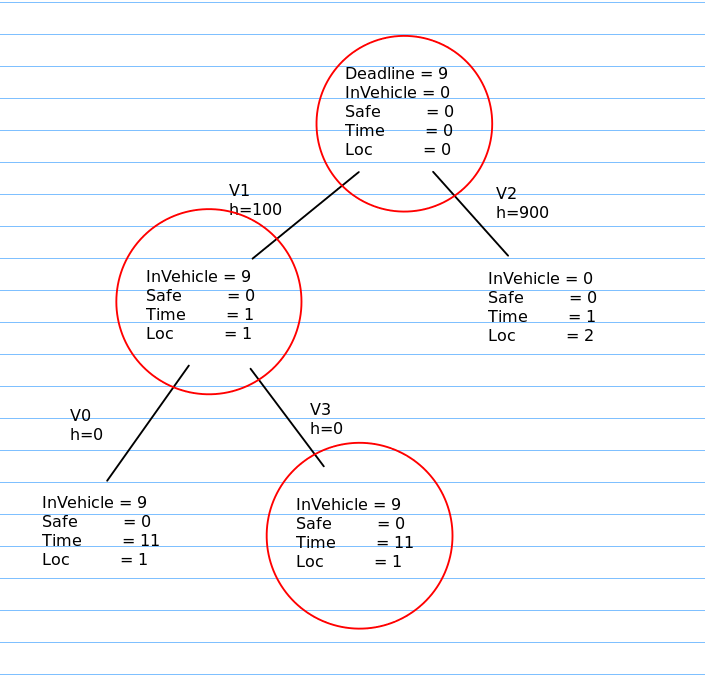
\includegraphics[width=0.5\linewidth]{q2a}
		\caption{Greedy agent expansions}
		\label{fig:q2a}
	\end{figure}
	
	
	\subsection{$ A^* $}
	Opposed to the greedy agent, the $ A^* $ agent will provide an optimal solution since the heuristic is admissible. Since, the heuristic is extremely optimistic the $ A^* $ agent will perform much more expansions than he would have needed if the heuristic was better.
	
	The $ A^* $ agent takes into account the time took to get to this state, and if a goal state is reached it adds the number of unsaved  people.
	\begin{equation}\label{eq:g_val}
		g_{v_i\rightarrow v_j}=
		\begin{cases}
		g[v_i] + w_{v_iv_j},& t + w_{v_iv_j} < T_{deadline}\\
		g[v_i] + w_{v_iv_j} + 100\times UnsavedPeople,& else\\
		\end{cases}
	\end{equation} 
	The agent adds the $ g $ value with the $ h $ value to decide which node to expand.
	
	Fig. \ref{fig:q2b} shows the expansion tree of the $ A^* $ agent. It can be seen that the agent has 11\footnote{The state $ V_0 $ with f=902 was not expanded since it is assumed there is a checking for loops to avoid expanding already visited states.} expansions to find the optimal path, which is $ V_0\rightarrow V_2\rightarrow V_3\rightarrow V_2\rightarrow V_0$. 

	
	\begin{figure}
		\centering
		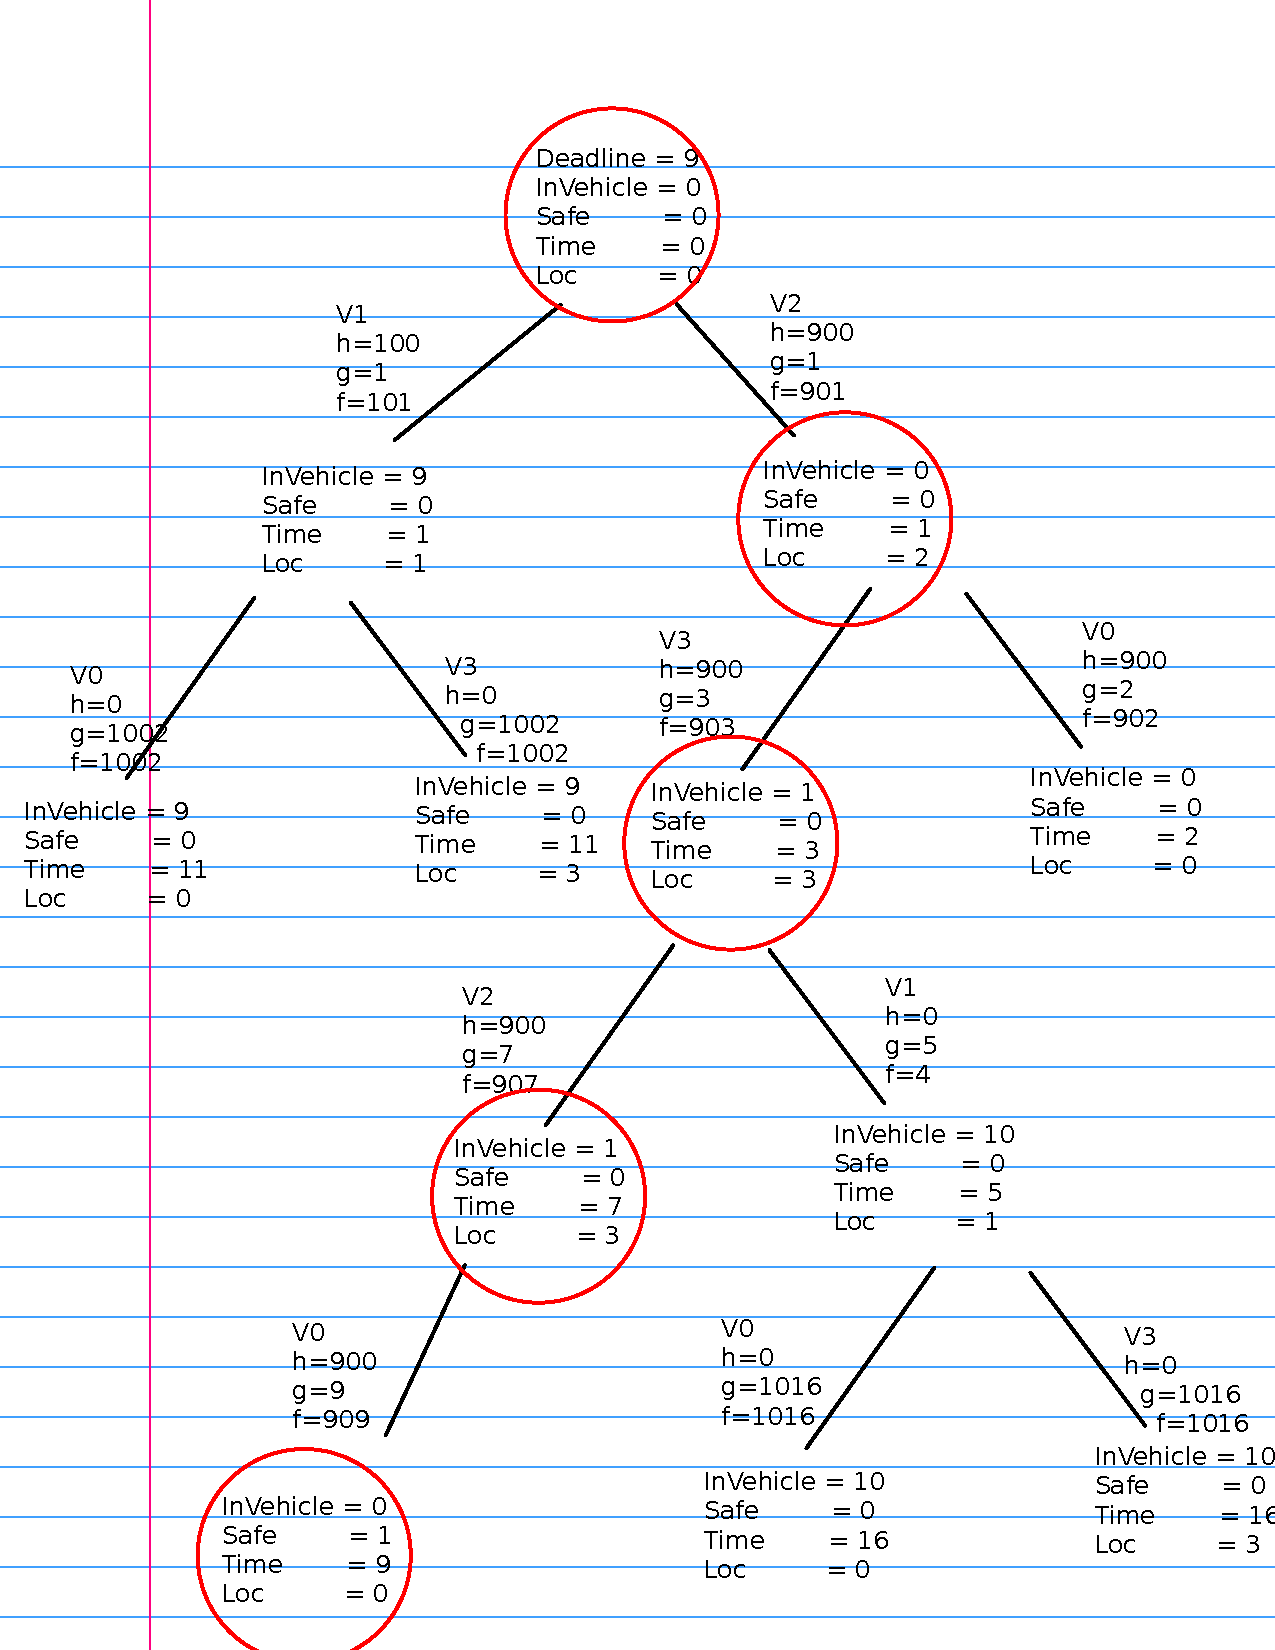
\includegraphics[width=0.5\linewidth]{q2_b}
		\caption{$ A^* $ agent expansions}
		\label{fig:q2b}
	\end{figure}

	\subsection{Real-time $ A^* $}
	
	This agent is similar to the $ A^* $ agent, however, it stops after 2 expansions and makes a decision. Fig~\ref{fig:q2c1} shows the first two expansions of the agent. It can be seen that in this case, the same result state is achieved as with the the $ A^* $ agent. After the agent reached $ V_3 $ the agent expanded up to two more nodes, as shown in Fig.~\ref{fig:q2c2}.
	\begin{figure}
		\centering
		\begin{subfigure}[b]{0.4\textwidth}
			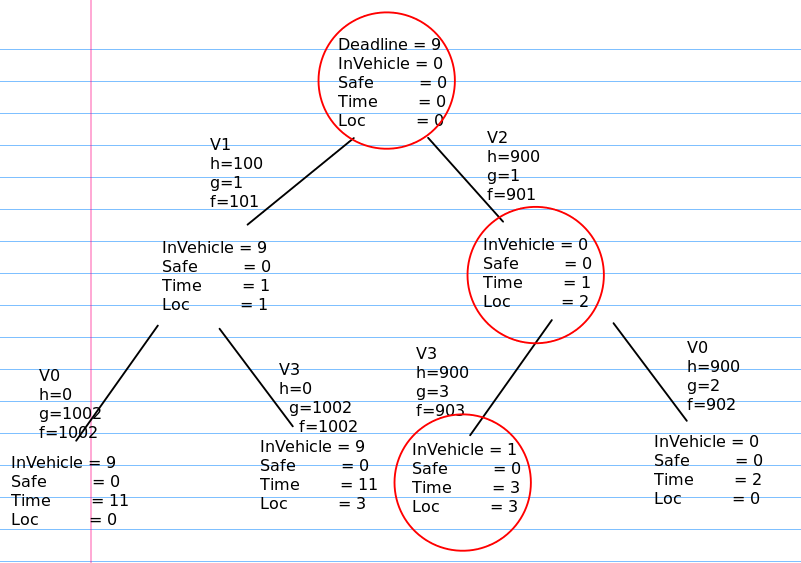
\includegraphics[width=\textwidth]{q2_c_1}
			\caption{Real-Time $ A^* $ agent first 2 expansions.}
			\label{fig:q2c1}
		\end{subfigure}
		\begin{subfigure}[b]{0.4\textwidth}
			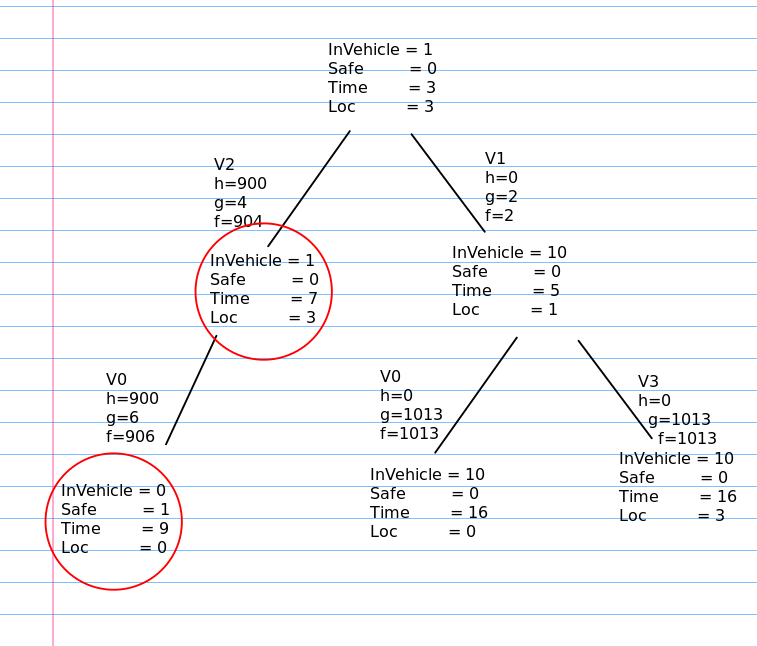
\includegraphics[width=\textwidth]{q2_c_2}
			\caption{Real-Time $ A^* $ agent second 2 expansions.}
			\label{fig:q2c2}
		\end{subfigure}
	
	\end{figure}

	\subsection{$ h=2 * h' $}
	Since $ h' $ multiplied the number of people by a large number, it does not matter if this large number is $ X $ or $ 2*X $. Therefore, all of the results will remain the same, and the heuristic is still admissible.
	
	\section{Game trees}
	
	
	\section{Game-tree search - alpha-beta pruning}
	
	
	\section{Propositional logic}
	
	
	
	\section{FOL and situation calculus}
	
	
	
	
%	\section{Game trees - 10$\%$}
%	\begin{tikzpicture}
%	
%	\node[draw,scale=0,label=left:A] (a_label) at (0,7) {};
%	\node[draw,scale=0,label=left:CHANCE] (c_label) at (0,6) {};
%	\node[draw,scale=0,label=left:B] (b_label) at (0,5) {};
%	\node[draw,scale=0,label=left:C] (c_label) at (0,4) {};
%	
%	\node[draw,fill=black,circle,scale=0.3] (a) at (7,7) {};
%	
%	\node[draw,circle,scale=0.7] (ch1) at (1.5,6) {};
%	\node[draw,circle,scale=0.7] (ch2) at (4,6) {};
%	\node[draw,circle,scale=0.7] (ch3) at (7,6) {};
%	\node[draw,circle,scale=0.7] (ch4) at (10,6) {};
%	\node[draw,circle,scale=0.7] (ch5) at (14,6) {};
%	
%	\node[draw,fill=black,circle,scale=0.3] (b1) at (1,5) {};
%	\node[draw,fill=black,circle,scale=0.3] (b2) at (2,5) {};
%	\node[draw,fill=black,circle,scale=0.3] (b3) at (4,5) {};
%	\node[draw,fill=black,circle,scale=0.3] (b4) at (7,5) {};
%	\node[draw,fill=black,circle,scale=0.3] (b5) at (10,5) {};
%	\node[draw,fill=black,circle,scale=0.3] (b6) at (14,5) {};
%	
%	\node[draw,fill=black,circle,scale=0.3] (c1) at (1,4) {};
%	\node[draw,fill=black,circle,scale=0.3] (c2) at (2,4) {};
%	\node[draw,fill=black,circle,scale=0.3] (c3) at (3,4) {};
%	\node[draw,fill=black,circle,scale=0.3] (c4) at (5.5,4) {};
%	\node[draw,fill=black,circle,scale=0.3] (c5) at (7,4) {};
%	\node[draw,fill=black,circle,scale=0.3] (c6) at (9,4) {};
%	\node[draw,fill=black,circle,scale=0.3] (c7) at (11.5,4) {};
%	\node[draw,fill=black,circle,scale=0.3] (c8) at (14,4) {};
%	
%	
%	\node[draw,fill=black,circle,scale=0.3,label=below:(10-1-1)] (u1) at (0,3) {};
%	\node[draw,fill=black,circle,scale=0.3,label=below:(7-1-1)] (u2) at (1.2,3) {};
%	\node[draw,fill=black,circle,scale=0.3,label=below:(1-9-9)] (u3) at (2.4,3) {};
%	\node[draw,fill=black,circle,scale=0.3,label=below:(1-1-10)] (u4) at (3.6,3) {};
%	\node[draw,fill=black,circle,scale=0.3,label=below:(1-2-1)] (u5) at (4.8,3) {};
%	\node[draw,fill=black,circle,scale=0.3,label=below:(9-2-2)] (u6) at (6,3) {};
%	\node[draw,fill=black,circle,scale=0.3,label=below:(8-1-1)] (u7) at (7.2,3) {};
%	\node[draw,fill=black,circle,scale=0.3,label=below:(9-9-9)] (u8) at (8.4,3) {};
%	\node[draw,fill=black,circle,scale=0.3,label=below:(1-1-10)] (u9) at (9.6,3) {};
%	\node[draw,fill=black,circle,scale=0.3,label=below:(1-2-1)] (u10) at (11.5,3) {};
%	\node[draw,fill=black,circle,scale=0.3,label=below:(10-1-4)] (u12) at (13.3,3) {};
%	\node[draw,fill=black,circle,scale=0.3,label=below:(1-1-5)] (u13) at (14.6,3) {};
%	
%	\draw [->]
%	(a) edge[anchor=south] node {b} (ch1) 
%	(a) edge[anchor=north] node {a} (ch2) 
%	(a) edge[anchor=west] node {e} (ch3) 
%	(a) edge[anchor=north] node {c} (ch4) 
%	(a) edge[anchor=south] node {d} (ch5) 
%	
%	(ch1) edge[anchor=east] node {0.5} (b1) 
%	(ch1) edge[anchor=west] node {0.5} (b2) 
%	(ch2) edge[anchor=west] node {1} (b3) 
%	(ch3) edge[anchor=west] node {1} (b4) 
%	(ch4) edge[anchor=west] node {1} (b5) 
%	(ch5) edge[anchor=west] node {1} (b6) 
%	
%	(b1) edge (c1) 
%	(b2) edge (c2) 
%	(b3) edge (c3) 
%	(b3) edge (c4) 
%	(b4) edge (c5) 
%	(b5) edge (c6) 
%	(b5) edge (c7) 
%	(b6) edge (c8) 
%	
%	(c1) edge (u1) 
%	(c2) edge (u2) 
%	(c3) edge (u3) 
%	(c3) edge (u4) 
%	(c4) edge (u5) 
%	(c4) edge (u6) 
%	(c5) edge (u7) 
%	(c6) edge (u8) 
%	(c6) edge (u9) 
%	(c7) edge (u10) 
%	(c8) edge (u12) 
%	(c8) edge (u13) 
%	;
%	
%	\end{tikzpicture}
%	
%	\subsection{Each agent out for itself, and they cannot communicate}
%	
%	\begin{tikzpicture}
%	
%	\node[draw,scale=0,label=left:A] (a_label) at (0,7) {};
%	\node[draw,scale=0,label=left:CHANCE] (c_label) at (0,6) {};
%	\node[draw,scale=0,label=left:B] (b_label) at (0,5) {};
%	\node[draw,scale=0,label=left:C] (c_label) at (0,4) {};
%	
%	\node[draw,fill=black,circle,scale=0.3,label=above:(9-2-2)] (a) at (7,7) {};
%	
%	\node[draw,circle,scale=0.7,label=above:(8.5-1-1)] (ch1) at (1.5,6) {};
%	\node[draw,circle,scale=0.7,label=right:(9-2-2)] (ch2) at (4,6) {};
%	\node[draw,circle,scale=0.7,label=right:(8-1-1)] (ch3) at (7,6) {};
%	\node[draw,circle,scale=0.7,label=right:(1-2-1)] (ch4) at (10,6) {};
%	\node[draw,circle,scale=0.7,label=right:(1-1-5)] (ch5) at (14,6) {};
%	
%	\node[draw,fill=black,circle,scale=0.3,label=below:(10-1-1)] (b1) at (1,5) {};
%	\node[draw,fill=black,circle,scale=0.3,label=below:(7-1-1)] (b2) at (2,5) {};
%	\node[draw,fill=black,circle,scale=0.3,label=right:(9-2-2)] (b3) at (4,5) {};
%	\node[draw,fill=black,circle,scale=0.3,label=right:(8-1-1)] (b4) at (7,5) {};
%	\node[draw,fill=black,circle,scale=0.3,label=right:(1-2-1)] (b5) at (10,5) {};
%	\node[draw,fill=black,circle,scale=0.3,label=right:(1-1-5)] (b6) at (14,5) {};
%	
%	\node[draw,fill=black,circle,scale=0.3,label=below:(10-1-1)] (c1) at (1,4) {};
%	\node[draw,fill=black,circle,scale=0.3,label=below:(7-1-1)] (c2) at (2,4) {};
%	\node[draw,fill=black,circle,scale=0.3,label=right:(1-1-10)] (c3) at (3,4) {};
%	\node[draw,fill=black,circle,scale=0.3,label=above:(9-2-2)] (c4) at (5.5,4) {};
%	\node[draw,fill=black,circle,scale=0.3,label=right:(8-1-1)] (c5) at (7,4) {};
%	\node[draw,fill=black,circle,scale=0.3,label=right:(1-1-10)] (c6) at (9,4) {};
%	\node[draw,fill=black,circle,scale=0.3,label=above:(1-2-1)] (c7) at (11.5,4) {};
%	\node[draw,fill=black,circle,scale=0.3,label=right:(1-1-5)] (c8) at (14,4) {};
%	
%	\node[draw,fill=black,circle,scale=0.3,label=below:(10-1-1)] (u1) at (0,3) {};
%	\node[draw,fill=black,circle,scale=0.3,label=below:(7-1-1)] (u2) at (1.2,3) {};
%	\node[draw,fill=black,circle,scale=0.3,label=below:(1-9-9)] (u3) at (2.4,3) {};
%	\node[draw,fill=black,circle,scale=0.3,label=below:(1-1-10)] (u4) at (3.6,3) {};
%	\node[draw,fill=black,circle,scale=0.3,label=below:(1-2-1)] (u5) at (4.8,3) {};
%	\node[draw,fill=black,circle,scale=0.3,label=below:(9-2-2)] (u6) at (6,3) {};
%	\node[draw,fill=black,circle,scale=0.3,label=below:(8-1-1)] (u7) at (7.2,3) {};
%	\node[draw,fill=black,circle,scale=0.3,label=below:(9-9-9)] (u8) at (8.4,3) {};
%	\node[draw,fill=black,circle,scale=0.3,label=below:(1-1-10)] (u9) at (9.6,3) {};
%	\node[draw,fill=black,circle,scale=0.3,label=below:(1-2-1)] (u10) at (11.5,3) {};
%	\node[draw,fill=black,circle,scale=0.3,label=below:(10-1-4)] (u12) at (13.3,3) {};
%	\node[draw,fill=black,circle,scale=0.3,label=below:(1-1-5)] (u13) at (14.6,3) {};
%	
%	\draw [->]
%	(a) edge[anchor=south] node {b} (ch1) 
%	(a) edge[anchor=north,line width=1pt, red] node {a} (ch2) 
%	(a) edge[anchor=west] node {e} (ch3) 
%	(a) edge[anchor=north] node {c} (ch4) 
%	(a) edge[anchor=south] node {d} (ch5) 
%	
%	(ch1) edge[anchor=east] node {0.5} (b1) 
%	(ch1) edge[anchor=west] node {0.5} (b2) 
%	(ch2) edge[anchor=west] node {1} (b3) 
%	(ch3) edge[anchor=west] node {1} (b4) 
%	(ch4) edge[anchor=west] node {1} (b5) 
%	(ch5) edge[anchor=west] node {1} (b6) 
%	
%	(b1) edge (c1) 
%	(b2) edge (c2) 
%	(b3) edge (c3) 
%	(b3) edge (c4) 
%	(b4) edge (c5) 
%	(b5) edge (c6) 
%	(b5) edge (c7) 
%	(b6) edge (c8) 
%	
%	(c1) edge (u1) 
%	(c2) edge (u2) 
%	(c3) edge (u3) 
%	(c3) edge (u4) 
%	(c4) edge (u5) 
%	(c4) edge (u6) 
%	(c5) edge (u7) 
%	(c6) edge (u8) 
%	(c6) edge (u9) 
%	(c7) edge (u10) 
%	(c8) edge (u12) 
%	(c8) edge (u13) 
%	;
%	
%	\end{tikzpicture}
%	
%	\subsection{Paranoid assumption: B and C are against A}
%	
%	\begin{tikzpicture}
%	
%	\node[draw,scale=0,label=left:A] (a_label) at (0,7) {};
%	\node[draw,scale=0,label=left:CHANCE] (c_label) at (0,6) {};
%	\node[draw,scale=0,label=left:B] (b_label) at (0,5) {};
%	\node[draw,scale=0,label=left:C] (c_label) at (0,4) {};
%	
%	\node[draw,fill=black,circle,scale=0.3,label=above:(8.5-1-1)] (a) at (7,7) {};
%	
%	\node[draw,circle,scale=0.7,label=above:(8.5-1-1)] (ch1) at (1.5,6) {};
%	\node[draw,circle,scale=0.7,label=right:(1-2-1)] (ch2) at (4,6) {};
%	\node[draw,circle,scale=0.7,label=right:(8-1-1)] (ch3) at (7,6) {};
%	\node[draw,circle,scale=0.7,label=right:(1-2-1)] (ch4) at (10,6) {};
%	\node[draw,circle,scale=0.7,label=right:(1-1-5)] (ch5) at (14,6) {};
%	
%	\node[draw,fill=black,circle,scale=0.3,label=below:(10-1-1)] (b1) at (1,5) {};
%	\node[draw,fill=black,circle,scale=0.3,label=below:(7-1-1)] (b2) at (2,5) {};
%	\node[draw,fill=black,circle,scale=0.3,label=right:(1-2-1)] (b3) at (4,5) {};
%	\node[draw,fill=black,circle,scale=0.3,label=right:(8-1-1)] (b4) at (7,5) {};
%	\node[draw,fill=black,circle,scale=0.3,label=right:(1-2-1)] (b5) at (10,5) {};
%	\node[draw,fill=black,circle,scale=0.3,label=right:(1-1-5)] (b6) at (14,5) {};
%	
%	\node[draw,fill=black,circle,scale=0.3,label=below:(10-1-1)] (c1) at (1,4) {};
%	\node[draw,fill=black,circle,scale=0.3,label=below:(7-1-1)] (c2) at (2,4) {};
%	\node[draw,fill=black,circle,scale=0.3,label=right:(1-1-10)] (c3) at (3,4) {};
%	\node[draw,fill=black,circle,scale=0.3,label=above:(1-2-1)] (c4) at (5.5,4) {};
%	\node[draw,fill=black,circle,scale=0.3,label=right:(8-1-1)] (c5) at (7,4) {};
%	\node[draw,fill=black,circle,scale=0.3,label=right:(1-1-10)] (c6) at (9,4) {};
%	\node[draw,fill=black,circle,scale=0.3,label=above:(1-2-1)] (c7) at (11.5,4) {};
%	\node[draw,fill=black,circle,scale=0.3,label=right:(1-1-5)] (c8) at (14,4) {};
%	
%	\node[draw,fill=black,circle,scale=0.3,label=below:(10-1-1)] (u1) at (0,3) {};
%	\node[draw,fill=black,circle,scale=0.3,label=below:(7-1-1)] (u2) at (1.2,3) {};
%	\node[draw,fill=black,circle,scale=0.3,label=below:(1-9-9)] (u3) at (2.4,3) {};
%	\node[draw,fill=black,circle,scale=0.3,label=below:(1-1-10)] (u4) at (3.6,3) {};
%	\node[draw,fill=black,circle,scale=0.3,label=below:(1-2-1)] (u5) at (4.8,3) {};
%	\node[draw,fill=black,circle,scale=0.3,label=below:(9-2-2)] (u6) at (6,3) {};
%	\node[draw,fill=black,circle,scale=0.3,label=below:(8-1-1)] (u7) at (7.2,3) {};
%	\node[draw,fill=black,circle,scale=0.3,label=below:(9-9-9)] (u8) at (8.4,3) {};
%	\node[draw,fill=black,circle,scale=0.3,label=below:(1-1-10)] (u9) at (9.6,3) {};
%	\node[draw,fill=black,circle,scale=0.3,label=below:(1-2-1)] (u10) at (11.5,3) {};
%	\node[draw,fill=black,circle,scale=0.3,label=below:(10-1-4)] (u12) at (13.3,3) {};
%	\node[draw,fill=black,circle,scale=0.3,label=below:(1-1-5)] (u13) at (14.6,3) {};
%	
%	\draw [->]
%	(a) edge[anchor=south,line width=1pt, red] node {b} (ch1) 
%	(a) edge[anchor=north] node {a} (ch2) 
%	(a) edge[anchor=west] node {e} (ch3) 
%	(a) edge[anchor=north] node {c} (ch4) 
%	(a) edge[anchor=south] node {d} (ch5) 
%	
%	(ch1) edge[anchor=east] node {0.5} (b1) 
%	(ch1) edge[anchor=west] node {0.5} (b2) 
%	(ch2) edge[anchor=west] node {1} (b3) 
%	(ch3) edge[anchor=west] node {1} (b4) 
%	(ch4) edge[anchor=west] node {1} (b5) 
%	(ch5) edge[anchor=west] node {1} (b6) 
%	
%	(b1) edge (c1) 
%	(b2) edge (c2) 
%	(b3) edge (c3) 
%	(b3) edge (c4) 
%	(b4) edge (c5) 
%	(b5) edge (c6) 
%	(b5) edge (c7) 
%	(b6) edge (c8) 
%	
%	(c1) edge (u1) 
%	(c2) edge (u2) 
%	(c3) edge (u3) 
%	(c3) edge (u4) 
%	(c4) edge (u5) 
%	(c4) edge (u6) 
%	(c5) edge (u7) 
%	(c6) edge (u8) 
%	(c6) edge (u9) 
%	(c7) edge (u10) 
%	(c8) edge (u12) 
%	(c8) edge (u13) 
%	;
%	
%	\end{tikzpicture}
%	
%	\subsection{B and C may agree on a deal if it is beneficial to both of them}
%	
%	\begin{tikzpicture}
%	
%	\node[draw,scale=0,label=left:A] (a_label) at (0,7) {};
%	\node[draw,scale=0,label=left:CHANCE] (c_label) at (0,6) {};
%	\node[draw,scale=0,label=left:B] (b_label) at (0,5) {};
%	\node[draw,scale=0,label=left:C] (c_label) at (0,4) {};
%	
%	\node[draw,fill=black,circle,scale=0.3,label=above:(9-9-9)] (a) at (7,7) {};
%	
%	\node[draw,circle,scale=0.7,label=above:(8.5-1-1)] (ch1) at (1.5,6) {};
%	\node[draw,circle,scale=0.7,label=right:(1-9-9)] (ch2) at (4,6) {};
%	\node[draw,circle,scale=0.7,label=right:(8-1-1)] (ch3) at (7,6) {};
%	\node[draw,circle,scale=0.7,label=right:(9-9-9)] (ch4) at (10,6) {};
%	\node[draw,circle,scale=0.7,label=right:(1-1-5)] (ch5) at (14,6) {};
%	
%	\node[draw,fill=black,circle,scale=0.3,label=below:(10-1-1)] (b1) at (1,5) {};
%	\node[draw,fill=black,circle,scale=0.3,label=below:(7-1-1)] (b2) at (2,5) {};
%	\node[draw,fill=black,circle,scale=0.3,label=right:(1-9-9)] (b3) at (4,5) {};
%	\node[draw,fill=black,circle,scale=0.3,label=right:(8-1-1)] (b4) at (7,5) {};
%	\node[draw,fill=black,circle,scale=0.3,label=right:(9-9-9)] (b5) at (10,5) {};
%	\node[draw,fill=black,circle,scale=0.3,label=right:(1-1-5)] (b6) at (14,5) {};
%	
%	\node[draw,fill=black,circle,scale=0.3,label=below:(10-1-1)] (c1) at (1,4) {};
%	\node[draw,fill=black,circle,scale=0.3,label=below:(7-1-1)] (c2) at (2,4) {};
%	\node[draw,fill=black,circle,scale=0.3,label=right:(1-9-9)] (c3) at (3,4) {};
%	\node[draw,fill=black,circle,scale=0.3,label=above:(9-2-2)] (c4) at (5.5,4) {};
%	\node[draw,fill=black,circle,scale=0.3,label=right:(8-1-1)] (c5) at (7,4) {};
%	\node[draw,fill=black,circle,scale=0.3,label=right:(9-9-9)] (c6) at (9,4) {};
%	\node[draw,fill=black,circle,scale=0.3,label=above:(1-2-1)] (c7) at (11.5,4) {};
%	\node[draw,fill=black,circle,scale=0.3,label=right:(1-1-5)] (c8) at (14,4) {};
%	
%	\node[draw,fill=black,circle,scale=0.3,label=below:(10-1-1)] (u1) at (0,3) {};
%	\node[draw,fill=black,circle,scale=0.3,label=below:(7-1-1)] (u2) at (1.2,3) {};
%	\node[draw,fill=black,circle,scale=0.3,label=below:(1-9-9)] (u3) at (2.4,3) {};
%	\node[draw,fill=black,circle,scale=0.3,label=below:(1-1-10)] (u4) at (3.6,3) {};
%	\node[draw,fill=black,circle,scale=0.3,label=below:(1-2-1)] (u5) at (4.8,3) {};
%	\node[draw,fill=black,circle,scale=0.3,label=below:(9-2-2)] (u6) at (6,3) {};
%	\node[draw,fill=black,circle,scale=0.3,label=below:(8-1-1)] (u7) at (7.2,3) {};
%	\node[draw,fill=black,circle,scale=0.3,label=below:(9-9-9)] (u8) at (8.4,3) {};
%	\node[draw,fill=black,circle,scale=0.3,label=below:(1-1-10)] (u9) at (9.6,3) {};
%	\node[draw,fill=black,circle,scale=0.3,label=below:(1-2-1)] (u10) at (11.5,3) {};
%	\node[draw,fill=black,circle,scale=0.3,label=below:(10-1-4)] (u12) at (13.3,3) {};
%	\node[draw,fill=black,circle,scale=0.3,label=below:(1-1-5)] (u13) at (14.6,3) {};
%	
%	\draw [->]
%	(a) edge[anchor=south] node {b} (ch1) 
%	(a) edge[anchor=north] node {a} (ch2) 
%	(a) edge[anchor=west] node {e} (ch3) 
%	(a) edge[anchor=north,line width=1pt, red] node {c} (ch4) 
%	(a) edge[anchor=south] node {d} (ch5) 
%	
%	(ch1) edge[anchor=east] node {0.5} (b1) 
%	(ch1) edge[anchor=west] node {0.5} (b2) 
%	(ch2) edge[anchor=west] node {1} (b3) 
%	(ch3) edge[anchor=west] node {1} (b4) 
%	(ch4) edge[anchor=west] node {1} (b5) 
%	(ch5) edge[anchor=west] node {1} (b6) 
%	
%	(b1) edge (c1) 
%	(b2) edge (c2) 
%	(b3) edge (c3) 
%	(b3) edge (c4) 
%	(b4) edge (c5) 
%	(b5) edge (c6) 
%	(b5) edge (c7) 
%	(b6) edge (c8) 
%	
%	(c1) edge (u1) 
%	(c2) edge (u2) 
%	(c3) edge (u3) 
%	(c3) edge (u4) 
%	(c4) edge (u5) 
%	(c4) edge (u6) 
%	(c5) edge (u7) 
%	(c6) edge (u8) 
%	(c6) edge (u9) 
%	(c7) edge (u10) 
%	(c8) edge (u12) 
%	(c8) edge (u13) 
%	;
%	
%	\end{tikzpicture}
%	
%	\subsection{A and C are partners aiming to maximize the sum of their scores}
%	
%	\begin{tikzpicture}
%	
%	\node[draw,scale=0,label=left:A] (a_label) at (0,7) {};
%	\node[draw,scale=0,label=left:CHANCE] (c_label) at (0,6) {};
%	\node[draw,scale=0,label=left:B] (b_label) at (0,5) {};
%	\node[draw,scale=0,label=left:C] (c_label) at (0,4) {};
%	
%	\node[draw,fill=black,circle,scale=0.3,label=above:(10-1-4)] (a) at (7,7) {};
%	
%	\node[draw,circle,scale=0.7,label=above:(8.5-1-1)] (ch1) at (1.5,6) {};
%	\node[draw,circle,scale=0.7,label=right:(9-2-2)] (ch2) at (4,6) {};
%	\node[draw,circle,scale=0.7,label=right:(8-1-1)] (ch3) at (7,6) {};
%	\node[draw,circle,scale=0.7,label=right:(9-9-9)] (ch4) at (10,6) {};
%	\node[draw,circle,scale=0.7,label=right:(10-1-4)] (ch5) at (14,6) {};
%	
%	\node[draw,fill=black,circle,scale=0.3,label=below:(10-1-1)] (b1) at (1,5) {};
%	\node[draw,fill=black,circle,scale=0.3,label=below:(7-1-1)] (b2) at (2,5) {};
%	\node[draw,fill=black,circle,scale=0.3,label=right:(9-2-2)] (b3) at (4,5) {};
%	\node[draw,fill=black,circle,scale=0.3,label=right:(8-1-1)] (b4) at (7,5) {};
%	\node[draw,fill=black,circle,scale=0.3,label=right:(9-9-9)] (b5) at (10,5) {};
%	\node[draw,fill=black,circle,scale=0.3,label=right:(10-1-4)] (b6) at (14,5) {};
%	
%	\node[draw,fill=black,circle,scale=0.3,label=below:(10-1-1)] (c1) at (1,4) {};
%	\node[draw,fill=black,circle,scale=0.3,label=below:(7-1-1)] (c2) at (2,4) {};
%	\node[draw,fill=black,circle,scale=0.3,label=right:(1-1-10)] (c3) at (3,4) {};
%	\node[draw,fill=black,circle,scale=0.3,label=above:(9-2-2)] (c4) at (5.5,4) {};
%	\node[draw,fill=black,circle,scale=0.3,label=right:(8-1-1)] (c5) at (7,4) {};
%	\node[draw,fill=black,circle,scale=0.3,label=right:(9-9-9)] (c6) at (9,4) {};
%	\node[draw,fill=black,circle,scale=0.3,label=above:(1-2-1)] (c7) at (11.5,4) {};
%	\node[draw,fill=black,circle,scale=0.3,label=right:(10-1-4)] (c8) at (14,4) {};
%	
%	\node[draw,fill=black,circle,scale=0.3,label=below:(10-1-1)] (u1) at (0,3) {};
%	\node[draw,fill=black,circle,scale=0.3,label=below:(7-1-1)] (u2) at (1.2,3) {};
%	\node[draw,fill=black,circle,scale=0.3,label=below:(1-9-9)] (u3) at (2.4,3) {};
%	\node[draw,fill=black,circle,scale=0.3,label=below:(1-1-10)] (u4) at (3.6,3) {};
%	\node[draw,fill=black,circle,scale=0.3,label=below:(1-2-1)] (u5) at (4.8,3) {};
%	\node[draw,fill=black,circle,scale=0.3,label=below:(9-2-2)] (u6) at (6,3) {};
%	\node[draw,fill=black,circle,scale=0.3,label=below:(8-1-1)] (u7) at (7.2,3) {};
%	\node[draw,fill=black,circle,scale=0.3,label=below:(9-9-9)] (u8) at (8.4,3) {};
%	\node[draw,fill=black,circle,scale=0.3,label=below:(1-1-10)] (u9) at (9.6,3) {};
%	\node[draw,fill=black,circle,scale=0.3,label=below:(1-2-1)] (u10) at (11.5,3) {};
%	\node[draw,fill=black,circle,scale=0.3,label=below:(10-1-4)] (u12) at (13.3,3) {};
%	\node[draw,fill=black,circle,scale=0.3,label=below:(1-1-5)] (u13) at (14.6,3) {};
%	
%	\draw [->]
%	(a) edge[anchor=south] node {b} (ch1) 
%	(a) edge[anchor=north] node {a} (ch2) 
%	(a) edge[anchor=west] node {e} (ch3) 
%	(a) edge[anchor=north] node {c} (ch4) 
%	(a) edge[anchor=south,line width=1pt, red] node {d} (ch5) 
%	
%	(ch1) edge[anchor=east] node {0.5} (b1) 
%	(ch1) edge[anchor=west] node {0.5} (b2) 
%	(ch2) edge[anchor=west] node {1} (b3) 
%	(ch3) edge[anchor=west] node {1} (b4) 
%	(ch4) edge[anchor=west] node {1} (b5) 
%	(ch5) edge[anchor=west] node {1} (b6) 
%	
%	(b1) edge (c1) 
%	(b2) edge (c2) 
%	(b3) edge (c3) 
%	(b3) edge (c4) 
%	(b4) edge (c5) 
%	(b5) edge (c6) 
%	(b5) edge (c7) 
%	(b6) edge (c8) 
%	
%	(c1) edge (u1) 
%	(c2) edge (u2) 
%	(c3) edge (u3) 
%	(c3) edge (u4) 
%	(c4) edge (u5) 
%	(c4) edge (u6) 
%	(c5) edge (u7) 
%	(c6) edge (u8) 
%	(c6) edge (u9) 
%	(c7) edge (u10) 
%	(c8) edge (u12) 
%	(c8) edge (u13) 
%	;
%	
%	\end{tikzpicture}
%	
%	\subsection{A is a firm believer in Murphy's laws: "mother nature is a b*!=h", and wants to
%		play absolutely safe.}
%	
%	\begin{tikzpicture}
%	
%	\node[draw,scale=0,label=left:A] (a_label) at (0,7) {};
%	\node[draw,scale=0,label=left:CHANCE] (c_label) at (0,6) {};
%	\node[draw,scale=0,label=left:B] (b_label) at (0,5) {};
%	\node[draw,scale=0,label=left:C] (c_label) at (0,4) {};
%	
%	\node[draw,fill=black,circle,scale=0.3,label=above:(8-1-1)] (a) at (7,7) {};
%	
%	\node[draw,circle,scale=0.7,label=above:(7-1-1)] (ch1) at (1.5,6) {};
%	\node[draw,circle,scale=0.7,label=right:(1-1-9)] (ch2) at (4,6) {};
%	\node[draw,circle,scale=0.7,label=right:(8-1-1)] (ch3) at (7,6) {};
%	\node[draw,circle,scale=0.7,label=right:(1-1-10)] (ch4) at (10,6) {};
%	\node[draw,circle,scale=0.7,label=right:(1-1-5)] (ch5) at (14,6) {};
%	
%	\node[draw,fill=black,circle,scale=0.3,label=below:(10-1-1)] (b1) at (1,5) {};
%	\node[draw,fill=black,circle,scale=0.3,label=below:(7-1-1)] (b2) at (2,5) {};
%	\node[draw,fill=black,circle,scale=0.3,label=right:(1-1-9)] (b3) at (4,5) {};
%	\node[draw,fill=black,circle,scale=0.3,label=right:(8-1-1)] (b4) at (7,5) {};
%	\node[draw,fill=black,circle,scale=0.3,label=right:(1-1-10)] (b5) at (10,5) {};
%	\node[draw,fill=black,circle,scale=0.3,label=right:(1-1-5)] (b6) at (14,5) {};
%	
%	\node[draw,fill=black,circle,scale=0.3,label=below:(10-1-1)] (c1) at (1,4) {};
%	\node[draw,fill=black,circle,scale=0.3,label=below:(7-1-1)] (c2) at (2,4) {};
%	\node[draw,fill=black,circle,scale=0.3,label=right:(1-1-9)] (c3) at (3,4) {};
%	\node[draw,fill=black,circle,scale=0.3,label=above:(1-2-1)] (c4) at (5.5,4) {};
%	\node[draw,fill=black,circle,scale=0.3,label=right:(8-1-1)] (c5) at (7,4) {};
%	\node[draw,fill=black,circle,scale=0.3,label=right:(1-1-10)] (c6) at (9,4) {};
%	\node[draw,fill=black,circle,scale=0.3,label=above:(1-2-1)] (c7) at (11.5,4) {};
%	\node[draw,fill=black,circle,scale=0.3,label=right:(1-1-5)] (c8) at (14,4) {};
%	
%	\node[draw,fill=black,circle,scale=0.3,label=below:(10-1-1)] (u1) at (0,3) {};
%	\node[draw,fill=black,circle,scale=0.3,label=below:(7-1-1)] (u2) at (1.2,3) {};
%	\node[draw,fill=black,circle,scale=0.3,label=below:(1-9-9)] (u3) at (2.4,3) {};
%	\node[draw,fill=black,circle,scale=0.3,label=below:(1-1-10)] (u4) at (3.6,3) {};
%	\node[draw,fill=black,circle,scale=0.3,label=below:(1-2-1)] (u5) at (4.8,3) {};
%	\node[draw,fill=black,circle,scale=0.3,label=below:(9-2-2)] (u6) at (6,3) {};
%	\node[draw,fill=black,circle,scale=0.3,label=below:(8-1-1)] (u7) at (7.2,3) {};
%	\node[draw,fill=black,circle,scale=0.3,label=below:(9-9-9)] (u8) at (8.4,3) {};
%	\node[draw,fill=black,circle,scale=0.3,label=below:(1-1-10)] (u9) at (9.6,3) {};
%	\node[draw,fill=black,circle,scale=0.3,label=below:(1-2-1)] (u10) at (11.5,3) {};
%	\node[draw,fill=black,circle,scale=0.3,label=below:(10-1-4)] (u12) at (13.3,3) {};
%	\node[draw,fill=black,circle,scale=0.3,label=below:(1-1-5)] (u13) at (14.6,3) {};
%	
%	\draw [->]
%	(a) edge[anchor=south] node {b} (ch1) 
%	(a) edge[anchor=north] node {a} (ch2) 
%	(a) edge[anchor=west,line width=1pt, red] node {e} (ch3) 
%	(a) edge[anchor=north] node {c} (ch4) 
%	(a) edge[anchor=south] node {d} (ch5) 
%	
%	(ch1) edge[anchor=east] node {0.5} (b1) 
%	(ch1) edge[anchor=west] node {0.5} (b2) 
%	(ch2) edge[anchor=west] node {1} (b3) 
%	(ch3) edge[anchor=west] node {1} (b4) 
%	(ch4) edge[anchor=west] node {1} (b5) 
%	(ch5) edge[anchor=west] node {1} (b6) 
%	
%	(b1) edge (c1) 
%	(b2) edge (c2) 
%	(b3) edge (c3) 
%	(b3) edge (c4) 
%	(b4) edge (c5) 
%	(b5) edge (c6) 
%	(b5) edge (c7) 
%	(b6) edge (c8) 
%	
%	(c1) edge (u1) 
%	(c2) edge (u2) 
%	(c3) edge (u3) 
%	(c3) edge (u4) 
%	(c4) edge (u5) 
%	(c4) edge (u6) 
%	(c5) edge (u7) 
%	(c6) edge (u8) 
%	(c6) edge (u9) 
%	(c7) edge (u10) 
%	(c8) edge (u12) 
%	(c8) edge (u13) 
%	;
%	
%	\end{tikzpicture}
	

\end{document}

